\chapter{\LaTeX{} Tutorial}
\label{cha:latex-tutorial}

\section{\TeX{} Units}
\label{sec:tex-units}

\begin{figure}[h]
  \centering
  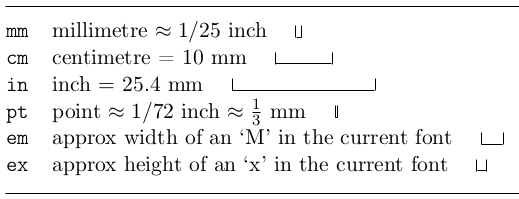
\includegraphics[width=.5\textwidth]{units}
  \caption{\TeX{} Units}
  \label{fig:tex-units}
\end{figure}

\section{Special characters}
\label{sec:special-characters}

The following 10 characters has special meanings in
\LaTeX{}.

\begin{center}
  \verb|& % $ # _ { } ~ ^ \|
\end{center}

Outside \textit{verb}, the first 7 should escaped by
\textit{backslash}. Of the last three, we use \LaTeX{} macros,
namely \verb|\textasciitilde|, \verb|\textasciicircum| and
\verb|\textbackslash|.

\begin{lstlisting}[language=TeX,caption={Special Characters},label={lst:special-characters}]
\& \% \$ \# \_ \{ \} \textasciitilde{} \textasciicircum{} \textbackslash{}
\end{lstlisting}

Specially, \LaTeX{} uses tilde \textasciitilde{} as a non-breaking space. You
would usually use non-breaking spaces for punctuation marks in
some languages, for units and currencies, for initials, etc.

\section{verbatim and verb}
\label{sec:verbatim-verb}

When to show raw text without \LaTeX{} command being executed, use
\textit{verbatim} environment or \textit{verb} command. Both have
an asterisk alternative like \verb|\begin{verbatim*}| and
  \verb|\verb*|. With extra *, \LaTeX{} will typewrite space as
\texttt{␣}.

You can't use \texttt{\textbackslash{}verb} in other command's
parameters. For example, this is not allowed:

\begin{lstlisting}[language=TeX,caption={Illegal verb}]
\href{https://tex.stackexchange.com/a/23653}{When should we use
  \verb|\begin{center}| instead of \verb|\centering|?}
\end{lstlisting}

Instead, we use
\href{https://tex.stackexchange.com/q/2790}{\texttt{\textbackslash{}texttt}}
and escape special characters \footnote{For instance, backslash
and \{.} like:

\begin{lstlisting}[language=TeX,caption={texttt}]
\href{https://tex.stackexchange.com/a/23653}{When should we use
\texttt{\textbackslash{}begin\{center\}} instead of \texttt{\textbackslash{}centering}?}
\end{lstlisting}

\section{item list}
\label{sec:item-list}

Using lists is quite straightforward and does not require you to
add any additional packages. For unordered list, \LaTeX{} provides
the \textit{itemize} environment and for ordered list there is the
\textit{emunerate} environment. With both environments, elements
should be declared beginning with \verb|\item| command. We can use
\verb|M-Enter| binding to insert this command automatically.

Take a look at unordered list\ref{lst:itemize-unordered-list}:

\begin{minipage}{.4\linewidth}
\begin{lstlisting}[label={lst:itemize-unordered-list},linewidth=.7\textwidth]
\begin{itemize}
\item One
\item HKUST
\item HUST
\end{itemize}
\end{lstlisting}  
\end{minipage}
\hfill
\framebox{
\begin{minipage}{0.4\linewidth}
  \begin{itemize}
  \item One
  \item HUST
  \item HKUST
  \end{itemize}
\end{minipage}
}

Here is an ordered list \ref{lst:enumerate-ordered-list}:

\begin{minipage}{.4\linewidth}
  \begin{enumerate}
  \item Jim
  \item Gray
    \begin{itemize}
    \item This is a
    \item nested unordered
    \item list within ordered list
    \end{itemize}
  \item Who are you?
  \end{enumerate}
\end{minipage}
\hfill{}
\begin{minipage}{.4\linewidth}
\begin{lstlisting}[label={lst:enumerate-ordered-list}]
\begin{enumerate}
\item Jim
\item Gray
  \begin{itemize}
  \item This is a
  \item nested unordered
  \item list within ordered list
  \end{itemize}
\item Who are you?
\end{enumerate}
\end{lstlisting}
\end{minipage}

\section{Code listings}
\label{sec:code-listings}

Although \textit{verb} and \textit{verbatim} enclose raw text,
they don't highlight source code like C, Java etc. This is where
\textit{listings} package come into
\href{https://en.wikibooks.org/wiki/LaTeX/Source_Code_Listings}{usage}.

To insert a code block, use \textit{lstlisting} environment like

\begin{center}
  \verb|\begin{lstlisting}[language=bash,caption={Bash},frame=single]|
\end{center}

Here is an example:

\begin{lstlisting}[language=bash,caption={Bash},frame=single]
#!/bin/bash
echo 'Hello, world!'
\end{lstlisting}

Furthermore,
\begin{lstlisting}[language=TeX,caption={Include code file},breaklines]
\lstinputlisting[language=C,frame=tb,basicstyle=\scriptsize\ttfamily]{helloworld.c}
\end{lstlisting}
command includes code source file:
\lstinputlisting[language=C,frame=single,
caption={C98}]{helloworld.c} This is useful when the code needs
updating frequently.

To prevent \textit{lstlisting} from breaking pages, we should wrap
it within \textit{minipage} environment as \ref{lst:table-floating}.

Sometimes, code line is too long to fit page width, leaving
tailing part out of page. We could modify \textit{basicstyle} to
one of \textit{footnotesize}, \textit{scriptsize} and
\textit{tiny}. Check long text line example
\ref{cha:too-big-fit}. For more options, read
\href{https://tug.org/texinfohtml/latex2e.html#Font-sizes}{Font
  Size} and \href{https://tex.stackexchange.com/q/24599}{font size
  and point (pt) relation}.

{\LARGE This is LARGE text} {\Huge while this is Huge}.

\section{Straight Quotes}
\label{sec:straight-quotes}

By default, \textit{listings} typesets both single and double as
\textit{back curve ones}.

We should import \textit{textcomp} package and \textit{fontenc}
package with \href{https://tex.stackexchange.com/a/677}{T1}
option. Then, enable \textit{upquote=true} for code block. Read
more at \href{https://tex.stackexchange.com/q/166790}{How can I
  get straight double quotes in listings?}

This method, however, is discouraged as \textit{fontenc} would
override the whole document \LaTeX{} font settings. The underlying
cause is \textit{serif (roman)} font. Default roman fonts does not
provide straight quotes. We should tell \textit{listings} to use
\textit{monospace} font instead by

\begin{center}
  \verb|\lstset{basicstyle=\ttfamily}|
\end{center}

Read more at
\href{https://tex.stackexchange.com/q/144396}{Consolas: Straight
  Quotes}.

\section{floating}
\label{sec:floating}

\subsection{Figure}
\label{sec:figure}

First, we import \textit{graphicx} package and then set
\textit{graphicspath} in preamble part:
\begin{lstlisting}[language=TeX,caption={graphicx}]
\usepackage{graphicx}
\graphicspath{{figs/}{./}}
\end{lstlisting}

\textit{graphicx} accepts EPS, PDF, PNG or JPEG
formats. \textit{graphicspath} defines a list of directories
relative to that of \textit{master.tex}. By this means, we can
access images anywhere without restriction like
\verb|\graphicspath{{../../img/}}|. The trailing slash cannot be
omitted.

Then, we use command \textit{includegraphics} like

\begin{center}
  \verb|\includegraphics[width=.5\textwidth,scale=0.1]{myimg}|
\end{center}

Notice that we do not write figure file extension. Here is the
output:
\begin{center}
  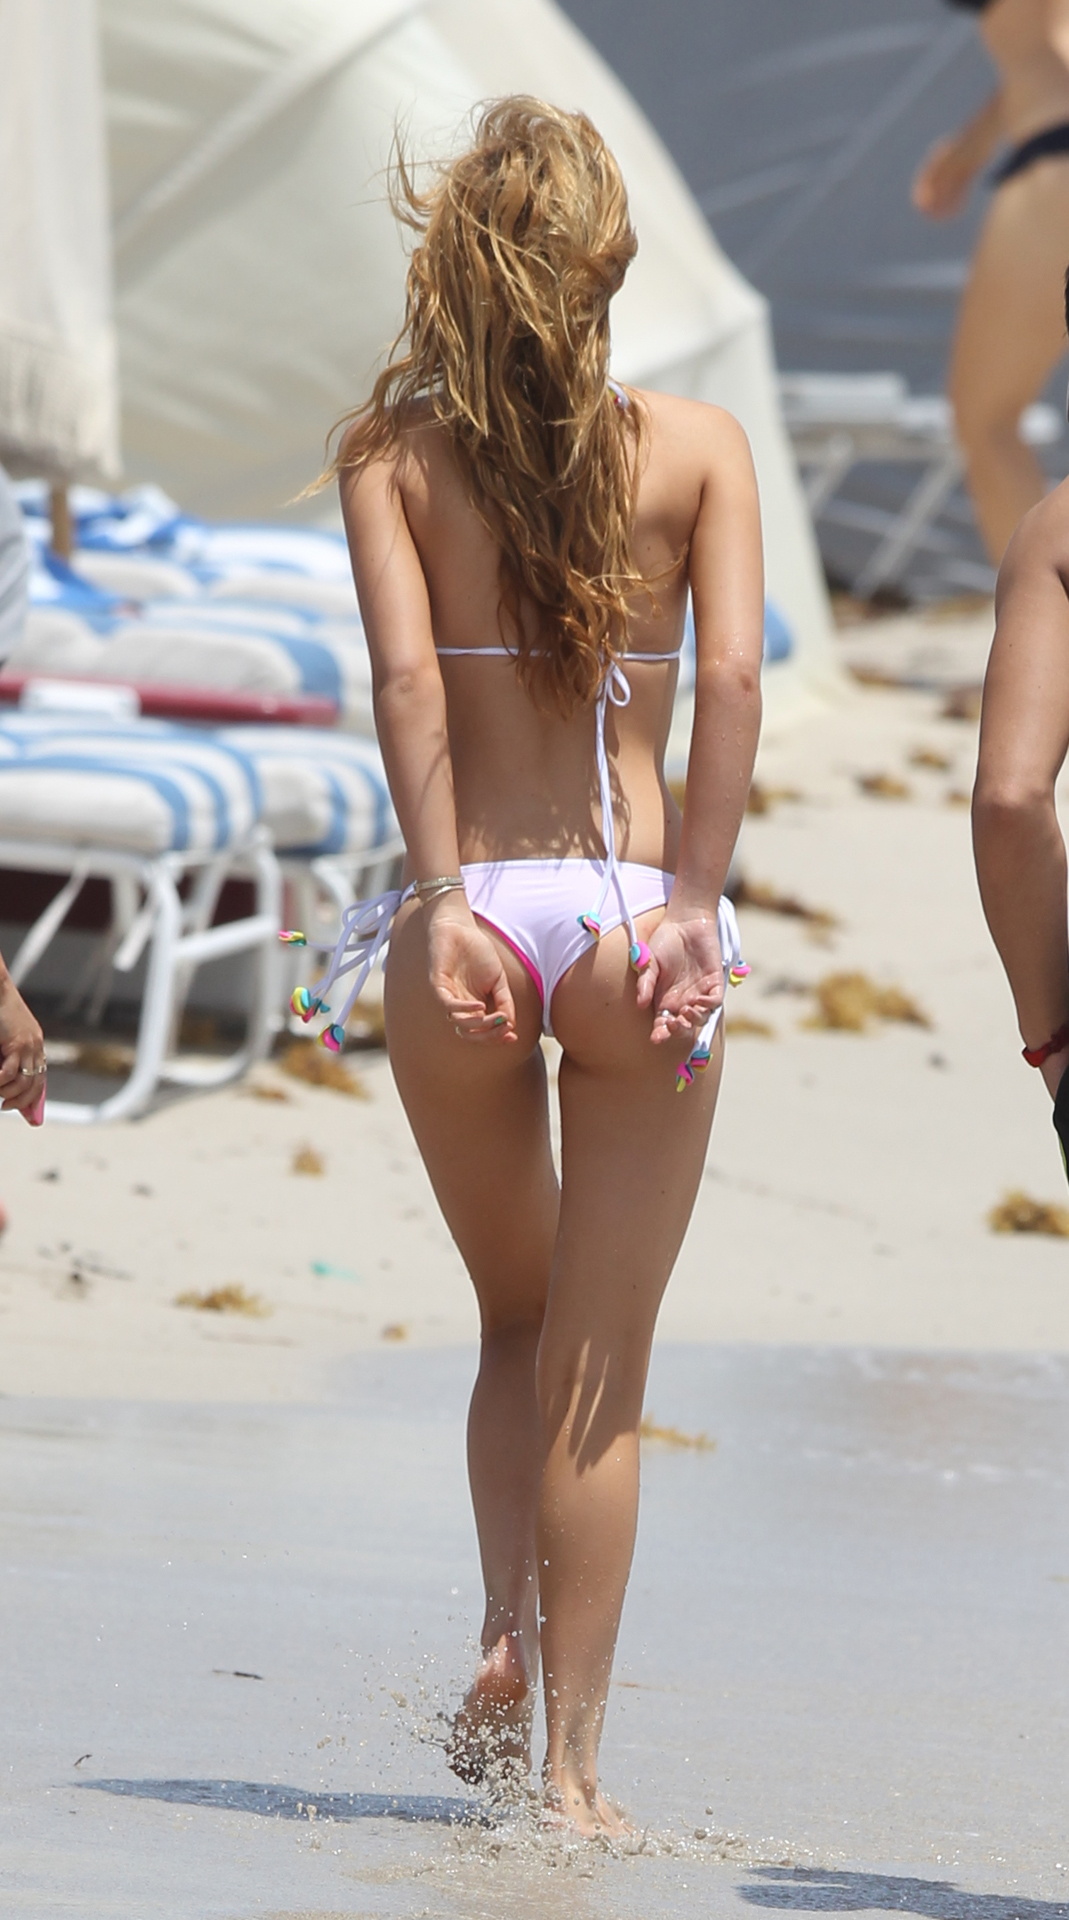
\includegraphics[width=.5\textwidth,scale=0.1]{leg}
\end{center}

With bare \textit{includegraphics}, if remaining space within current
page does not hold the figure, \LaTeX{} would start a new page
instead, leaving current page partially emtpy. The method is to
wrap it with \textit{figure} environment:

\begin{minipage}[top]{1.0\linewidth}
\begin{lstlisting}[language=TeX,caption={Figure Floating}]
\begin{figure}[tbp]
  \centering
  \includegraphics[width=\textwidth]{Boobs}
  \caption{Boobs}
  \label{fig:Boobs}
\end{figure}
\end{lstlisting}  
\end{minipage}

We call this technique as \textit{floating}. Apart from
\textit{placement specifier} benefits, we can define
\textit{label} and \textit{caption} within \textit{floating}
environment. Note that \verb|\label{}| command must come
\textbf{after} \verb|\caption{}| command since the reference
number is generated by \verb|\caption{}|. For details, refer to
\href{https://tex.stackexchange.com/a/32326}{Why does an
  environment's label have to appear after the caption?}.

The \verb|tbp| \footnote{\textit{tbp} is the default
  \textit{placement specifier}. We could set it to
  \textit{!htbp}.} specifies position of floating environment.

\begin{figure}[h]
  \centering
  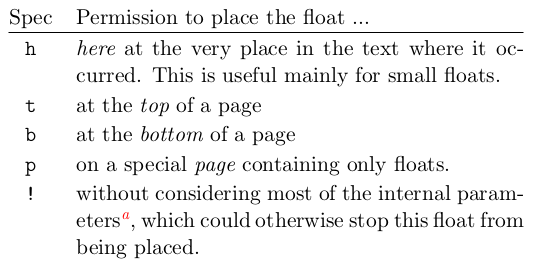
\includegraphics[width=.5\textwidth]{floating}
  \caption{Floating Placement Specifiers}
  \label{fig:placement-specifiers}
\end{figure}

Here is a nice boobs example \ref{fig:boobs}:

\begin{figure}[!htbp]
  \centering
  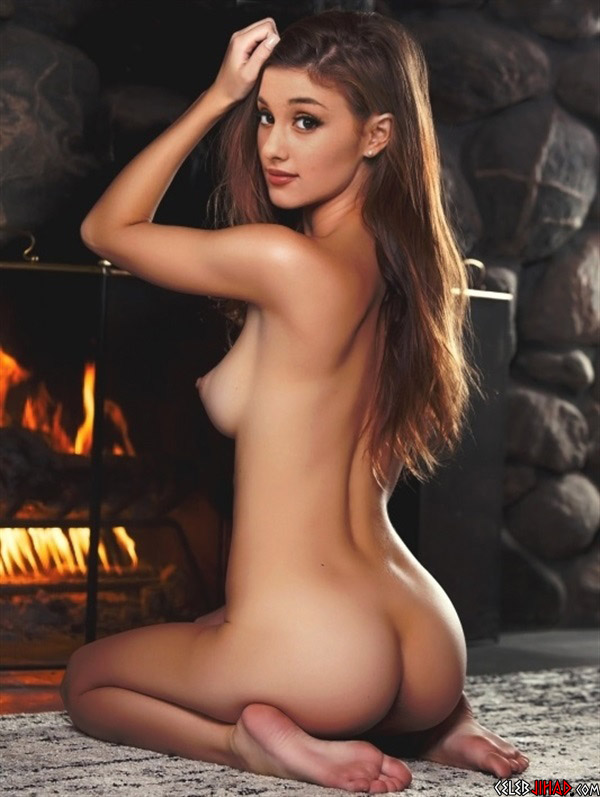
\includegraphics[scale=.3]{boobs}
  \caption{boobs}
  \label{fig:boobs}
\end{figure}

Sometimes, it's necessary to put figures side by side for clear
comparasion. We use \textit{subfigure} within \textit{figure} like
\ref{fig:three-girsl}. Please be noted that we add non-breakable
symbol \textasciitilde{} between \textit{subfigure} to leave
some space between figures.

\begin{figure}[tbp]
  \centering
  \begin{subfigure}[tbp]{0.3\linewidth}
    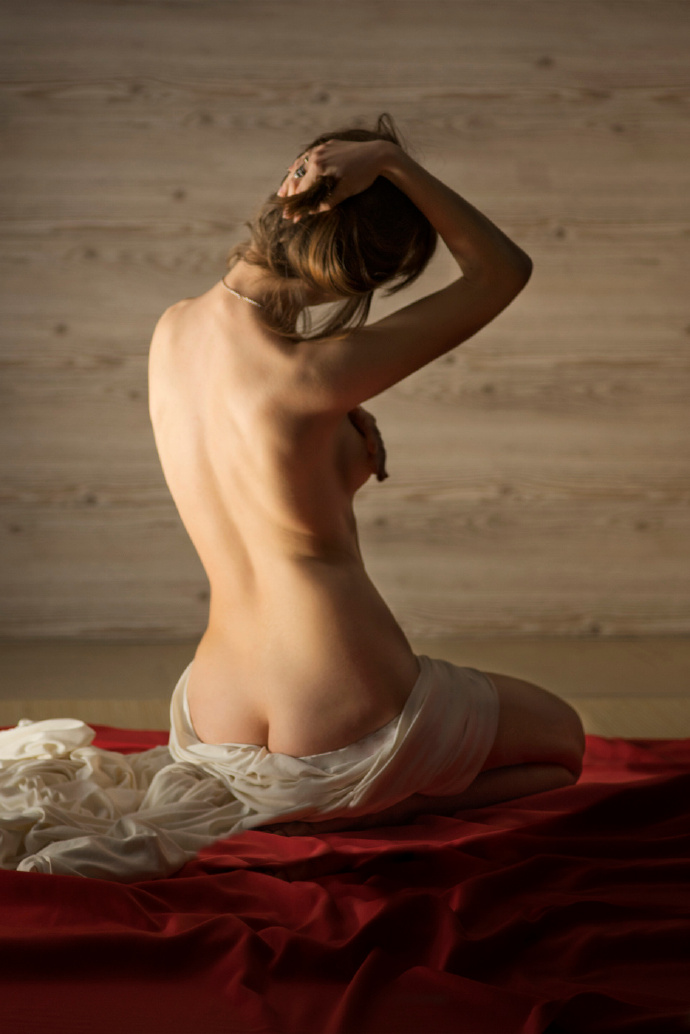
\includegraphics[width=\linewidth]{sub1}
    \caption{Girl A}
  \end{subfigure}
  ~
  \begin{subfigure}[tbp]{0.3\linewidth}
    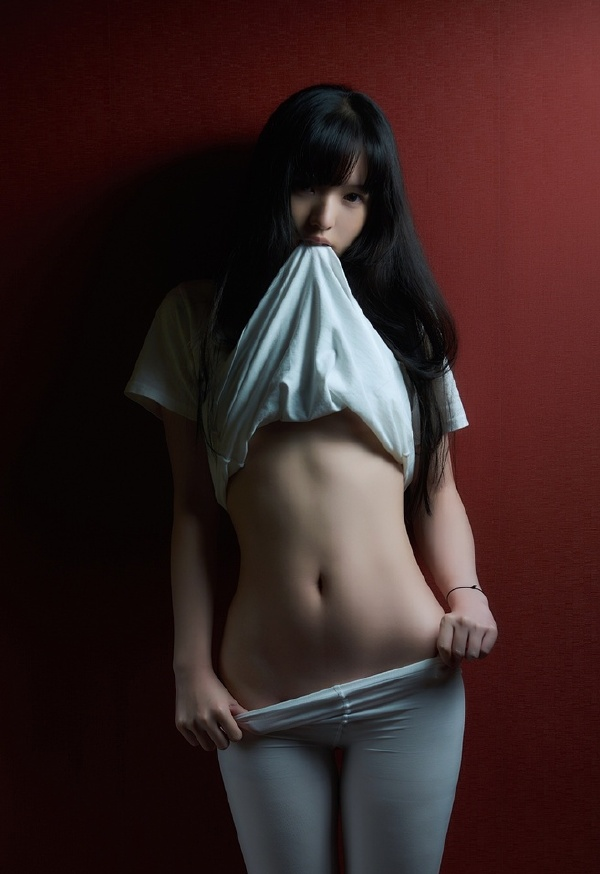
\includegraphics[width=\linewidth]{sub2}
    \caption{Girl B}
  \end{subfigure}
  ~
  \begin{subfigure}[tbp]{0.3\linewidth}
    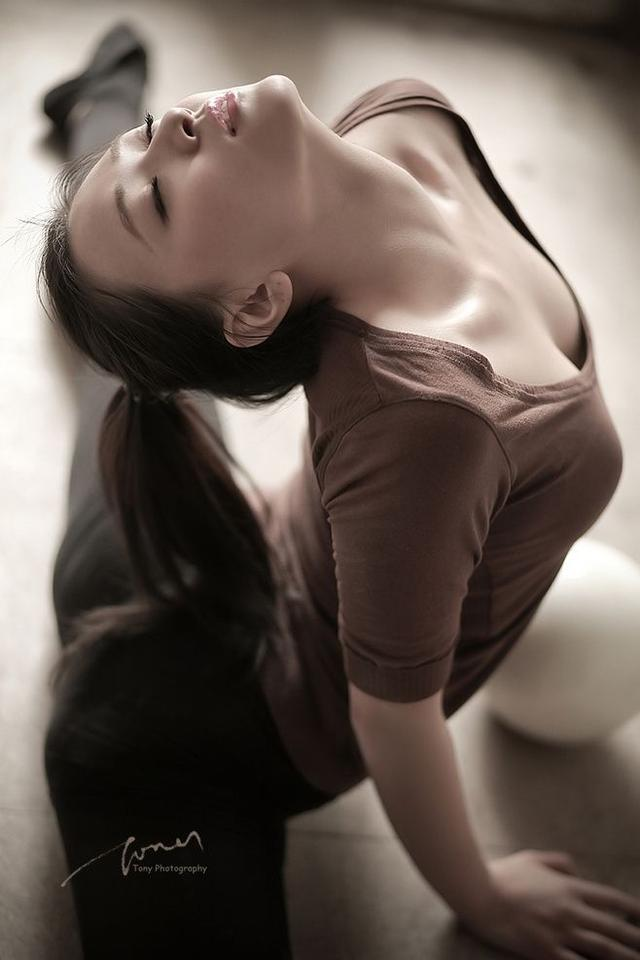
\includegraphics[width=\linewidth]{sub3}
    \caption{Girl C}
  \end{subfigure}
  \caption{Three Girls}
  \label{fig:three-girsl}
\end{figure}

\subsection{Table}
\label{sec:table}

Similarly, we can wrap \textit{tabular} within \textit{table}
environment to \textit{float} table \ref{tab:auctex-bindings} like
\ref{lst:table-floating}.

\begin{minipage}[top]{1.0\linewidth}
\begin{lstlisting}[language=TeX,caption={Table Floating},label={lst:table-floating}]
\begin{table}[!htbp]
  \centering
  \begin{tabular}{|l|r|}
    \hline{}
    Binding & Function \\ \hline \hline{}
    \verb|C-c C-e| & insert environment \\ \hline{}
    \verb|C-c C-s| & insert section \\ \hline{}
    \verb|C-c C-m| & macro (command) \\ \hline{}
    \verb|M-return| & another item \\ \hline{}
    \verb|C-c C-c| & compile \LaTeX{} \\ \hline{}
    \verb|C-c C-v| & preview output \\ \hline{}
    \verb|C-c =| & show document layout by RefTeX \\ \hline{}
    \verb|C-c C-o C-b| & fold the buffer \\ \hline{}
    \verb|C-c C-o b| & unfold the buffer \\ \hline
  \end{tabular}
  \caption{AUCTeX Bindings}
  \label{tab:auctex-bindings}
\end{table}
\end{lstlisting}
\end{minipage}

In \textit{tabular} environment, we align column texts as
\textit{\textbf{l}eft}, \textit{\textbf{c}enter} and
\textit{\textbf{r}ight}. What about decimal number cell? Idealy,
we want to align numbers at dot, where package \textit{siunitx}
plays a role by \textbf{S} \ref{tab:number-alignment-at-dot}
alignment specifier.

\begin{lstlisting}[language=TeX,caption={Decimal Alignment},label={lst:decimal-alignment}]
\usepackage[round-mode=places,round-precision=3]{siunitx}
\end{lstlisting}

To make prettier table, we use package \textit{booktabs} which
provides \textit{toprule}, \textit{midrule} and
\textit{bottomrule} to override \footnote{It is not replace!} dull \textit{hline}.

\begin{table}[tbp]
  \centering
  \begin{tabular}{l|S|r}
    \toprule{}
    \textbf{List 1} & \textbf{Decimal 2} & \textbf{Letter 3} \\
    $\alpha$ & $\beta$ & $\gamma{}$ \\
    \midrule{}
    1 & 1385.1 & a \\
    2 & 3.0674 & b \\
    3 & 87.369 & c \\
    \bottomrule
  \end{tabular}
  \caption{Number Alignment at Dot}
  \label{tab:number-alignment-at-dot}
\end{table}

To make more complex tables, we can use package \textit{multirow}
and \textit{multirow} and \textit{multicolumn} environment
respectivelly.

When typesetting large tables, it is tedious and error-prone which
could be avoided by \textit{pgfplotstable} package that generate
tables from external \textit{.csv} file. Programs such as Excel,
OpenOffice Calc or even emacs org-mode can export data sheets as
\textit{.csv} files. The \textit{pgfplotstable template}
\ref{sec:pgfplotstable-template} generate table
\ref{table-automation-from-csv}.

\begin{table}[tbp]
  \centering{}
  \pgfplotstabletypeset[
    multicolumn names,
    col sep=comma,
    display columns/0/.style={
      column name=$Ampere$,
      column type={S},string type
    },
    display columns/1/.style={
      column name=$Voltage$,
      column type={S},string type
    },
    display columns/2/.style={
      column name=$Energy$,
      column type={S},string type
    },
    every head row/.style={
      before row={\toprule},
      after row={
        \si{\ampere} & \si{\volt} & \si{\joule} \\
        \midrule
      }
    },
    every last row/.style={
      after row=\bottomrule
    },
  ]{pgfplotstable.csv}
  \caption{Table automation from .csv file.}
  \label{table-automation-from-csv}
\end{table}

\subsection{Plot}
\label{sec:plot}

The \textit{pgfplots} package is a powerful tool, based on
\textit{tikz} package, dedicated to create scientific
graphs. Similar to \textit{pgfplotstable}, \textit{pgfplots} can
read date from \textit{.csv} file.

Since \textit{pgfplots} is based on \textit{tikz}, the
\textit{axis} environment should be enclosed within
\textit{tikzpicture} environment. Template
\ref{lst:pgfplots-template} generates plot
\ref{fig:pgfplots-by-table-csv-file}.

\begin{figure}[!ht]
  \centering
  \begin{tikzpicture}
    \begin{axis}[
      width = \linewidth, % Scale the plot to \linewidth
      grid = major, grid style = dashed,
      xlabel = Voltage $U$, ylabel = Currency $I$, % Set the labels
      x unit = \si{\volt}, y unit = \si{\ampere}, % Set the respective units
      % axis lines = left % only display the left and bottom axes
      legend style = { at = {(0.5,-0.2)}, anchor = north }, % Put the legend below the plot
      x tick label style = { rotate = 90, anchor = east } % Display labels sideways
      ]
      % add a plot from table; you select the columns by using the
      % actual column header name in the .csv file
      \addplot
      table[x=value 1,y=value 2,col sep=comma]{pgfplots.csv};
      \legend{$U$ - $I$}
      % add another plot
      \addplot
      {x^2 - 2*x + 1}; % add a tailing semicolon
      \addlegendentry{$x^2 - 2x + 1$} % use addlegendentry instead of legend
    \end{axis}
  \end{tikzpicture}
  \caption{pgfplots by table csv file}
  \label{fig:pgfplots-by-table-csv-file}
\end{figure}

\textit{addplot} plots 2D figure, for 3D, we use \textit{addplot3}
\ref{fig:pgfplots-3d}.

\begin{figure}[tbp]
  \centering
  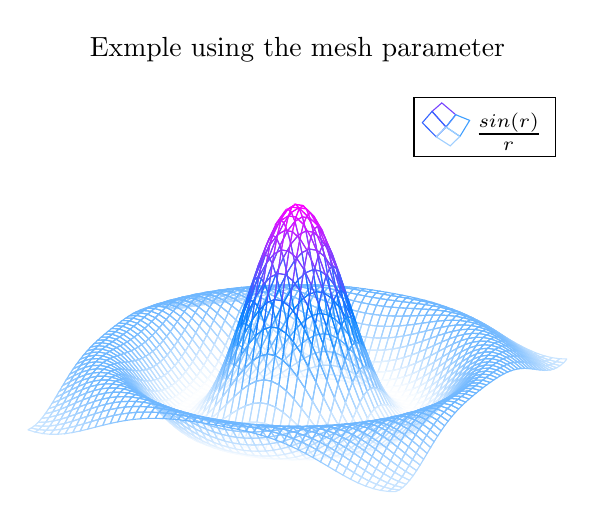
\begin{tikzpicture}
    \begin{axis}[
      title=Exmple using the mesh parameter,
      hide axis,
      colormap/cool,
      ]
      \addplot3[ mesh, samples=50, domain=-8:8, ]
      {sin(deg(sqrt(x^2+y^2)))/sqrt(x^2+y^2)};
      \addlegendentry{$\frac{sin(r)}{r}$}
      \end{axis}
  \end{tikzpicture}  
  \caption{pgfplots 3D}
  \label{fig:pgfplots-3d}
\end{figure}

Besides \textit{pgfplotstable} and \textit{pgfplots}, we could
aslo use \textit{tgiz} package or \textit{circuitkiz} to
\verb|\draw| pictures from within your LaTeX document.

\section{center and centering}
\label{sec:center-centering}

The main difference between \textit{center} environment and
\textit{centering} command is the former leave vertical space
before and after it while the later would not.

We usually use \verb|\centering{}| command within a group by curly
braces, figure, table, or
\verb|\begingroup \centering ... \endgroup|
\ref{lst:centering-within-braces}.

\begin{minipage}{1.0\linewidth}
\begin{lstlisting}[language=TeX,caption={centering within braces},label={lst:centering-within-braces}]
{\centering{centering require line break by \par, emtpy line or \\
before closing the group, otherwise text following the group wound
be centered either.}\\
}
\end{lstlisting}  
\end{minipage}

{\centering{centering require line break by \verb|\par|, emtpy
    line or \verb|\\| before closing the group, otherwise text
    following the group wound be centered either.}

} This line is not centered! Check
\href{https://tex.stackexchange.com/a/23653}{When should we use
  \texttt{\textbackslash{}begin\{center\}} instead of
  \texttt{\textbackslash{}centering}?} and
\href{http://texblog.net/latex-archive/floats/center-centering/}{center
  vs. centering}

\section{Math Equations}
\label{sec:math-equations}

To insert simple inline equation, we wrap it by \$ like
\verb|$c^2=a^2+b^2$|: $c^2=a^2+b^2$.

For tall or deep inline math expressions or sub expressions, we
can enclose them by \verb|\smash| command. This makes \LaTeX{}
ignore the height of these expressions. This keeps the line
spacing even like: \smash{$d_{e_{e_p}}$} followed by
\smash{$h^{i^{g^h}}$}.

This is an example without \verb|\smash|. You will find line space
is much bigger. A $d_{e_{e_p}}$ expression followed by a
$h^{i^{g^h}}$ one.

If we want equaton occupy a whole line, then wrap it by double
\$\$ or single bracket \verb|\[\]|. The equation will be centered
automatically.

\begin{lstlisting}[language=TeX,caption={Equation in new line},label={lst:equation-in-new-line}]
$$(1+x)^n=\sum_{k=0}^n\binom{n}{k}x^k$$
\end{lstlisting}

This is the output:
$$(1+x)^n=\sum_{k=0}^n\binom{n}{k}x^k$$
Let's have another example:
$$A_1+A_{100}$$

After examing the example above, you are recommended to tune
AUCTeX \ref{sec:auctex} configuration a little bit. Enable math
mode manually by \verb|C-c ~| or globally into Emacs startup:

\begin{lstlisting}[language=Lisp,caption={\LaTeX{} Math Mode},label={lst:latex-math-mode}]
(add-hook 'LaTeX-mode-hook 'LaTeX-math-mode)
\end{lstlisting}

We just prepend \verb|`| and type your desired math symbol. AUCTeX
automatically completes it. If given a prefix argument \verb|C-u|,
the symbol will be surrounded by dollar signs. For example, if you
type \verb|C-u ` b|, AUCTex will typeset \verb|$\beta$|. Read
AUCTex manual
\href{https://www.gnu.org/software/auctex/manual/auctex/Mathematics.html}{Entering
  Mathematics} for more details.

The \$ method by \TeX{} does provide some basic mathematics
features, but it is limited. we should
\verb|\usepackage{amsmath}|. What is more, we can
\verb|\usepackage{amssymb}| to make math symbols look shiny.

A bit further, we usually want to label and number a equation so
that we can refer to it somewhere else. Futhermore, it is better
for a long equation to occupy a new line. To do this, enclose
equation with \textit{equation} environment like
\eqref{eq:einstein}. Einstein says

\begin{equation}
  \label{eq:einstein}
  E = mc^2
\end{equation}

In order that multiple equations align properly at
\textit{ampersand \&}, we use \textit{align} or \textit{align*}
instead.  \eqref{eq:eq-alignment}. Each single equation must be
separated by \textit{linebreak \\\\}. The version with asterisk
just removes equation numbers.

\begin{align}
  \label{eq:multi-eqs}
  E &= mc^2 \\
  F &= ma
\end{align}

We use \textit{aligned} environment to align induction or
substitution lines of a single equation. Also, \textit{aligned}
should be enclosed within an equation environment.

\[
  \begin{aligned}[t]
    \label{eq:eq-alignment}
    f(x) &= x^2 \\
    \frac{1}{x} &= g(x) \\
    F(x) &= \int^a_b \frac{1}{\sqrt[3]{x}}
  \end{aligned}
\]

Compared to \textit{aligned}, \textit{align} and \textit{align*}
introduce extra space between lines to make the output
cleaner. Therefore, irrespective of single equation or multiple
equations, we'd better use \textit{align} and/or\textit{align*}.

\textit{matrix} environment must be enclosed by equation marker \&
or \textit{equatioin} environment.

\begin{lstlisting}[language=TeX,caption={Matrix},label={lst:matrix-marker}]
$
\begin{matrix}
  1 & 0 \\
  0 & 1
\end{matrix}
$
\end{lstlisting}

Similary, matrix breaks line by \verb|\\| and \& separates
columns. Here is a \textit{bmatrix} example:

\begin{equation}
  \label{eq:nn-matrix}
  A_{m,n} =
  \begin{bmatrix}
    a_{1,1} & a_{1,2} & \cdots & a_{1,n} \\
    a_{2,1} & a_{2,2} & \cdots & a_{2,n} \\
    \vdots & \vdots & \ddots & \vdots \\
    a_{n,1} & a_{n,2} & \cdots & a_{n,n}
  \end{bmatrix}  
\end{equation}

Recall that \$\$ or \verb|\[\]| let an equation placed on a new
line without label. They are equivalent to the
\verb|\begin{equation*}| environment.

\section{Document Structure}
\label{sec:file-structure}

\section{Boxes}
\label{sec:boxes}

Everything in \LaTeX{} is embedded in boxes, from letter to words,
\textit{tabular} to \textit{includegraphics}. TeX builds pages by
gluing \footnote{Squeeze and/or Stretch} boxes together according
to the default \TeX{} rules, default \LaTeX{} rules, or document
commands.

\href{https://en.wikibooks.org/wiki/LaTeX/Boxes}{Box} is of
paramount importance to get the base of \LaTeX{} typestting. Boxes
are placed relative to other boxes, while visible elements are
placed relative to the boxes which contain them.

Let's have a look at letter box illustration \ref{fig:letter-box}.

\begin{figure}[!htbp]
  \centering
  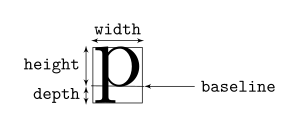
\includegraphics[width=.5\textwidth]{letter_box}
  \caption{Letter Box}
  \label{fig:letter-box}
\end{figure}

\verb|\parbox| is a box to wrap text into lines and lines are
broken into pages.

\begin{lstlisting}[language=TeX,caption={parbox box},label={lst:parbox-box}]
\parbox[pos][height][contentpos]{width}{text}
\end{lstlisting}

\textit{width} is a forced parameter to define box
width\footnote{It is \textbf{not} text width.} This argument can
be relative value like \verb|.8\textwidth|, absolute value like
\verb|5ex|, or \LaTeX{} and \TeX{} macros like
\verb|\width|. Similarly, we set \textit{height} in the same way.

\textit{pos} selects which \textit{baseline} of text to align with
neighbouring box. It can be \textbf{c}enter, \textbf{t}op, and
\textbf{b}ottom. For details, read the link above. Check
\ref{fig:parbox-baseline-alignment} for real effect.

\begin{figure}[!htbp]
  \centering
  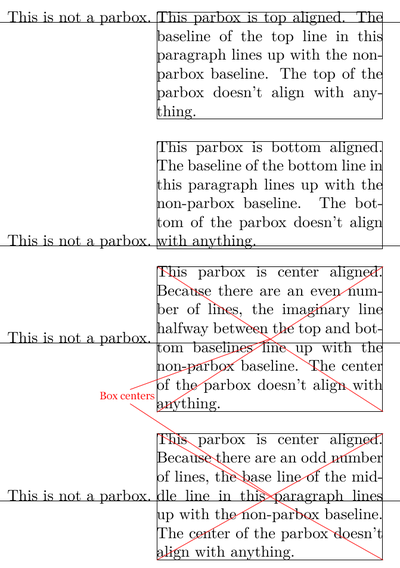
\includegraphics{parbox_baseline_alignment}
  \caption{parbox baseline alignment}
  \label{fig:parbox-baseline-alignment}
\end{figure}

This is a text line before \textit{parbox}
\parbox[t][2cm][t]{5cm}{This a text within \textit{parbox}. Please
  check text box and text alignment carefully.} This a tex line
after \textit{parbox}.

\textit{contentpos} positions the contents of the box within the
box which is straightforward. It only takes effect when box is
larger than texts it encases.

However, if the \textit{contentpos} is present and not the same as
\textit{pos} and \textit{pos} is not \textbf{c}enter, the
\verb|\parbox| will align at its borders instead of text baseline
\ref{fig:parbox-border-alignment}.

\begin{figure}[!htbp]
  \centering
  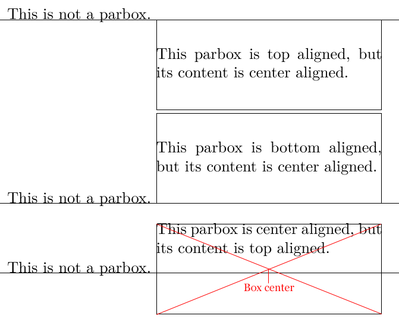
\includegraphics{parbox_border_alignment}
  \caption{parbox border alignment}
  \label{fig:parbox-border-alignment}
\end{figure}

This is a text line before \textit{parbox}
\parbox[t][2cm][b]{5cm}{This a text within \textit{parbox}. Please
  check text box and text alignment carefully.} This a tex line
after \textit{parbox}.

We also have \textit{minipage} environment box which is almost
identical to \verb|\parbox|. The difference between a
\textit{minipage} and a \verb|\parbox| is that you cannot use all
commands and environments inside a \verb|\parbox|, while almost
anything is possible in a \textit{minipage}. Hence, without
special requirement, we use the later one.

\begin{lstlisting}[language=TeX,caption={minipage box},label={lst:minipage-box}]
\begin{minipage}[pos][height][contentpos]{width} text \end{minipage}
\end{lstlisting}

Additionally, there are \textit{mbox}, \textit{makebox} and
\textit{framebox}.

In order to let multiple boxes stand side by side, we should make
sure their \textit{width} in total is less than 1, like
\ref{lst:enumerate-ordered-list}.

\subsection{input and include}
\label{sec:input-include}

Like other programming language, \LaTeX{} supports splitting large
document into different parts and
\href{https://tex.stackexchange.com/a/250}{importing} them
individually.

Use \verb|\include{filename}| in the \textit{document body} to
insert the contents of another file named
\textit{filename.tex}. Note that \LaTeX{} will start a new page
before processing the material input from
\textit{filename.tex}. \textit{include} is commonly used for
\textit{chapter} section.

\textit{include}'s sibling command
\verb|\includeonly{filename1,filename2,...}| is used in
\textit{preamble} part to insert only a subset of
\textit{included} files.

Alternatively, \verb|\input{filename}| is allowed in both
\textit{preamble} and \textit{body} parts. It does not start a new
page like \textit{include} but allow recursive \textit{include}
which is impossible for \textit{include}.

No matter which you choose, please omit \LaTeX{} file extension
\textit{.tex}.

\subsection{biblatex biber}
\label{sec:biblatex-biber}

Generally speaking, \textit{biblatex} and \textit{natbib} are
packages that handle \LaTeX{} citations in \textit{.tex} source
file. However, reference entries are stored separately in external
\textit{.bib} file. Hence, we require an intermediate tool to
format \textit{.bib} into \textit{.tex} source. That's when we
meet \textit{biber} and \textit{bibtex} which are named as
\textit{biblatex backend}.

Firstly, we should use \textit{biblatex} package:
\verb|\usepackage[backend=biber]{biblatex}|
and point out the external \textit{.bib} file to import:
\verb|\addbibresource{myref.bib}| in preamble part. Do not omit
\textit{.bib} extension.

Secondly, in the end of \LaTeX{} source (but before
\verb|\end{document}|), we print all reference entries:
\verb|\printbibliography[heading=bibintotoc]|.

Then, cite as you go. Before that, we should have a look at
\href{https://www.sharelatex.com/learn/Bibliography_management_in_LaTeX#The_bibliography_file}{\textit{.tex}
format}. The bibliography files must have the standard
\textit{bibtex} syntax. Here is a reference entry:
\begin{center}
\begin{lstlisting}[caption={BibTeX entry sample}]
@article{einstein,
    author = "Albert Einstein",
    title = "{Zur Elektrodynamik bewegter K{\"o}rper}. ({German})
    [{On} the electrodynamics of moving bodies]",
    journal = "Annalen der Physik",
    volume = "322",
    number = "10",
    pages = "891--921",
    year = "1905",
    DOI = "http://dx.doi.org/10.1002/andp.19053221004",
    keywords = "physics"
}
\end{lstlisting}
\end{center}

\verb|@article| tells the reference is an article. We also have
\verb|@book|, \verb|online| etc. \textit{einstein} is the
reference label that we will \textit{cite} with: \verb|\cite{einstein}|.

\subsection{RefTeX}
\label{sec:reftex}

RefTeX has been bundled and pre-installed with Emacs since version
20.2. We just add to Emacs:
\begin{lstlisting}[language=Lisp,caption={Enable RefTeX}]
; with AUCTeX LaTeX mode
(add-hook 'LaTeX-mode-hook 'turn-on-reftex)
; with Emacs latex mode
(add-hook 'latex-mode-hook 'turn-on-reftex)
\end{lstlisting}

To make cross-reference clickable (i.e. table of contents), use
package \textit{hyperref}.

Although \verb|C-c C-m| can prompt for \verb|\cite| command, we'd
better use
\href{https://www.gnu.org/software/auctex/manual/reftex.html}{RefTeX}
instead. RefTeX wraps itself round four LaTeX macros:
\verb|\label|, \verb|\ref|, \verb|\cite|, and \verb|\index|,
making the process more intelligent.

As mentioned earlier, RefTeX binding \verb|C-c =| displays document layout
in a newly created buffer.

To \textit{cite}, we use \verb|C-c [| binding and press \verb|^M|
\footnote{It is Enter key or Ctrl and letter `m', not Emacs Meta Alt
key.}. Afterwards, type a \textit{regular expression} to search
reference entries in \textit{.bib} file. Please be noted, there is
no completion prompt for \textit{regular expression}.

For reference to objects (i.e. figures) within the document, we
use \verb|C-c )|. For details, please visit
\href{https://www.gnu.org/software/auctex/manual/reftex/RefTeX-in-a-Nutshell.html}{RefTeX
  in a Nutshell}. RefTeX seems not to support \textit{href} to
URLs.

Sometimes, RefTeX cannot find newly created labels, references
etc. We should tell it to \textit{reftex-parse-all} or
\textit{reftex-parse-one} to parse \LaTeX{} source files.

%%% Local Variables:
%%% mode: latex
%%% TeX-master: "main"
%%% End:
